\begin{table*}[!tb]
\caption{Comparison on four planar sequences (top) and two volumes (bottom). All entries are local measurements on shared inputs. Bold/underline mark best/second distinct values among the merge tree maps; ties share emphasis. The Hilbert and Morton curves are references in fixed orientations and are not ranked.}
\label{tab:quantitative-final}
\footnotesize
\setlength{\tabcolsep}{1.5pt}
\renewcommand{\arraystretch}{0.85}
\begin{tabular*}{\textwidth}{@{\extracolsep{\fill}}l*{10}{c}lccc@{}}
\toprule
\multirow{2}{*}{Dataset} & \multicolumn{2}{c}{Hilbert} & \multicolumn{2}{c}{Morton} & \multicolumn{3}{c}{TMTM} & \multicolumn{3}{c}{ST-MTM} & \multicolumn{4}{c}{AnchorMTM (ours)} \\
\cmidrule(lr){2-3}\cmidrule(lr){4-5}\cmidrule(lr){6-8}\cmidrule(lr){9-11}\cmidrule(lr){12-15}
 & SNS$\downarrow$ & TW$\uparrow$ & SNS$\downarrow$ & TW$\uparrow$ & SNS$\downarrow$ & TW$\uparrow$ & NPE$\downarrow$ & SNS$\downarrow$ & TW$\uparrow$ & NPE$\downarrow$ & Mode & SNS$\downarrow$ & TW$\uparrow$ & NPE$\downarrow$ \\
\midrule
\multirow{2}{*}{Ring} & \multirow{2}{*}{$0.1252$} & \multirow{2}{*}{$0.9048$} & \multirow{2}{*}{$0.1489$} & \multirow{2}{*}{$0.7619$} & \multirow{2}{*}{$0.1970$} & \multirow{2}{*}{$0.4762$} & \multirow{2}{*}{$0.1756$} & \multirow{2}{*}{$\mathbf{0.0794}$} & \multirow{2}{*}{$0.9286$} & \multirow{2}{*}{$0.2463$} & Exact & $0.1485$ & $0.8571$ & $\underline{0.0471}$ \\
 &  &  &  &  &  &  &  &  &  &  & Balanced & $\underline{0.1334}$ & $0.8571$ & $\mathbf{0.0395}$ \\
\multirow{2}{*}{Wildfires} & \multirow{2}{*}{$0.1883$} & \multirow{2}{*}{$0.8303$} & \multirow{2}{*}{$0.1304$} & \multirow{2}{*}{$0.8758$} & \multirow{2}{*}{$0.1220$} & \multirow{2}{*}{$0.8444$} & \multirow{2}{*}{$0.2280$} & \multirow{2}{*}{$\mathbf{0.0186}$} & \multirow{2}{*}{$0.8968$} & \multirow{2}{*}{$0.3180$} & Exact & $\underline{0.0426}$ & $0.9136$ & $\underline{0.0131}$ \\
 &  &  &  &  &  &  &  &  &  &  & Balanced & $0.0447$ & $0.8989$ & $\mathbf{0.0116}$ \\
\multirow{2}{*}{Storms} & \multirow{2}{*}{$0.1290$} & \multirow{2}{*}{$0.7403$} & \multirow{2}{*}{$0.1180$} & \multirow{2}{*}{$0.7251$} & \multirow{2}{*}{$0.1420$} & \multirow{2}{*}{$0.6515$} & \multirow{2}{*}{$0.5753$} & \multirow{2}{*}{$\mathbf{0.0608}$} & \multirow{2}{*}{$0.8377$} & \multirow{2}{*}{$0.4579$} & Exact & $0.0790$ & $0.8463$ & $\underline{0.0399}$ \\
 &  &  &  &  &  &  &  &  &  &  & Balanced & $\underline{0.0743}$ & $0.8766$ & $\mathbf{0.0140}$ \\
\multirow{2}{*}{PM2.5} & \multirow{2}{*}{$0.2386$} & \multirow{2}{*}{$0.8887$} & \multirow{2}{*}{$0.1760$} & \multirow{2}{*}{$0.8277$} & \multirow{2}{*}{$0.3018$} & \multirow{2}{*}{$0.7781$} & \multirow{2}{*}{$0.5241$} & \multirow{2}{*}{$\underline{0.1897}$} & \multirow{2}{*}{$\mathbf{0.8224}$} & \multirow{2}{*}{$0.5577$} & Exact & $0.1964$ & $\underline{0.7884}$ & $\underline{0.1390}$ \\
 &  &  &  &  &  &  &  &  &  &  & Balanced & $\mathbf{0.1636}$ & $0.7657$ & $\mathbf{0.0468}$ \\
\midrule
\multirow{2}{*}{Cylinder} & \multirow{2}{*}{$0.2798$} & \multirow{2}{*}{$0.7902$} & \multirow{2}{*}{$0.2071$} & \multirow{2}{*}{$0.8008$} & \multirow{2}{*}{$0.2956$} & \multirow{2}{*}{$0.8017$} & \multirow{2}{*}{$0.4769$} & \multirow{2}{*}{$0.1346$} & \multirow{2}{*}{$\underline{0.8989}$} & \multirow{2}{*}{$0.5160$} & Exact & $\underline{0.1097}$ & $0.8136$ & $\underline{0.0918}$ \\
 &  &  &  &  &  &  &  &  &  &  & Balanced & $\mathbf{0.0405}$ & $\mathbf{0.8998}$ & $\mathbf{0.0133}$ \\
\multirow{2}{*}{Tangaroa} & \multirow{2}{*}{$0.3429$} & \multirow{2}{*}{$0.9222$} & \multirow{2}{*}{$0.3627$} & \multirow{2}{*}{$0.8893$} & \multirow{2}{*}{$0.5255$} & \multirow{2}{*}{$0.6701$} & \multirow{2}{*}{$0.3866$} & \multirow{2}{*}{$0.1655$} & \multirow{2}{*}{$\underline{0.8137}$} & \multirow{2}{*}{$0.3286$} & Exact & $\underline{0.1518}$ & $0.8061$ & $\underline{0.0861}$ \\
 &  &  &  &  &  &  &  &  &  &  & Balanced & $\mathbf{0.1364}$ & $\mathbf{0.8476}$ & $\mathbf{0.0465}$ \\
\bottomrule
\end{tabular*}
\vspace{2pt}
\begin{minipage}{\textwidth}\footnotesize The three benchmark inputs are our reconstructions (Section~\ref{sec:experiments}); TMTM and ST-MTM are scored on them from the runs that give their NPE (Supplementary Section~S4.2). TW needs enough features per frame: only 1/40, 4/32 and 11/744 frames are eligible on Ring, Wildfires and Storms, so TW is listed but not ranked there. Mode applies only to AnchorMTM. The curves break the tree, and NPE is not given for them because a curve index corresponds to no spatial direction. PM2.5 uses 744 shared-input local frames (TW $k=1$, full coverage); its Balanced mode uses the fixed exploratory 5\% case budget, without validation-set budget selection. ST-MTM uses the Storms preset with start frame 0. Volumes: streamwise $x$ reference, TW $k=1$; Cylinder Exact counts merge levels within $2\varepsilon_0$ as equal (NPE 0.1364 if they are kept distinct; Supplementary Table~S5); Balanced is 1\% (Cylinder) and 9\% (Tangaroa) by the planar rule, attaining 0.99\% and 9.0\% merge error. ST-MTM was not proposed for volumes; its volume rows are our adaptation (Section~\ref{sec:experiments}).\end{minipage}

\end{table*}


\section{Evaluation}\label{sec:experiments}
The evaluation follows the argument of the paper. We first test the bounds and use them to measure how much of the error of existing maps the tree actually forces; this evidence does not depend on what AnchorMTM optimizes. We then ask whether the anchored axis reaches its goal and what that costs in relative geometry and temporal behavior, examine how a merge budget changes individual frames, and close with case studies that set anchored maps beside their source fields.

\subsection{Data and Measures}
\paragraph{Data.} The four planar sequences are Ring (40 frames), Wildfires (32) and Storms (744), our reconstructions of the ST-MTM benchmark~\cite{STMTM:2026} at its per-frame persistence fractions, because its processed arrays are not available, and hourly PM$_{2.5}$ over northern China in January 2017 (744 frames, 5\% persistence)~\cite{Kong:2021:CAQRA}; Storms uses ERA5 sea-level-pressure anomalies~\cite{Hersbach:2020:ERA5} and Wildfires aggregated fire radiative power~\cite{Franke:2021:1DP}. We omit the Gaussian sequence of that benchmark, which has three features per frame and no conflict between hierarchy and position. The volumes are the flow past a square cylinder (102 frames of the $Q$-criterion, 2\% persistence)~\cite{Camarri:2005:Cylinder,Weinkauf:SquareCylinder} and the Tangaroa ship wake (201 speed fields, absolute persistence 0.2)~\cite{Popinet:2004:Tangaroa}. Within each comparison, all methods share the fields, trees, identities and references.

\paragraph{Compared maps.} TMTM and ST-MTM keep the tree but define no origin or direction for their axis, so each is reflected once per sequence to agree with the reference. ST-MTM was proposed for planar data, and its authors make no claim about volumes; because it is the only existing map that optimizes relative geometry and its inputs do not depend on the dimension, we include our own 3-D adaptation, with 3-D distances and the method's general parameters and without tuning (Supplementary Section~S4.2). The Hilbert and Morton space-filling curves are references for neighborhood quality only: they order all samples of the domain and break the tree, and a curve index corresponds to no spatial direction, so we report no NPE for them and do not rank them.

\paragraph{Measures.} Table~\ref{tab:measures} lists the measures. NPE is our own: AnchorMTM optimizes it and TMTM and ST-MTM do not, so it shows whether the anchoring goal is reached and does not rank the maps in general. The bound and the measures from prior work do not depend on it. SNS and TW compare anchor distances with support-centroid distances. TW needs enough features per frame and is not ranked on Ring, Wildfires and Storms, where only 1, 4 and 11 frames are eligible.

\begin{table}[!tb]
\centering
\caption{Measures of the evaluation. Lower is better, except for TW (higher) and TD (no preferred value, since features do move).}
\label{tab:measures}
\footnotesize
\setlength{\tabcolsep}{3pt}
\renewcommand{\arraystretch}{0.95}
\begin{tabular}{@{}lp{.68\columnwidth}l@{}}
\toprule
Measure & Meaning & Source\\
\midrule
$\nu^*$ & Smallest order error the tree forces (Eq.~\ref{eq:nu}) & this paper\\
NROE & Order error: least worst displacement of a leaf order (Eq.~\ref{eq:nroe}) & this paper\\
NPE & Worst displacement of the drawn map (Eq.~\ref{eq:nroe}) & this paper\\
Merge & Largest change of a displayed merge level (Eq.~\ref{eq:dtop}) & \cite{Munch:2019:LINF}\\
SNS & Scale-normalized stress of distances & \cite{Smelser:2025:Scale}\\
TW & Trustworthiness of neighbors & \cite{Venna:2001:NP}\\
TD & Summed displayed motion of matched anchors & \cite{STMTM:2026}\\
ME & Share of feature pairs whose displayed approach or separation contradicts the true one & --\\
\bottomrule
\end{tabular}
\end{table}

\paragraph{Modes.} Exact uses $\varepsilon=0$. Balanced uses a positive budget selected once from 1--10\% on the first chronological quarter of each benchmark input (1, 5 and 10\%); PM$_{2.5}$ uses a fixed 5\%. The volumes use the default configuration, the same Balanced rule and the streamwise axis of both flows as a supplied direction (Section~\ref{sec:reference-model}; Supplementary Section~S4.7 gives Tangaroa along its motion); Table~S1 lists the other settings and runtimes: ordering and placement take 0.15--3.32\,s per benchmark sequence and 200\,s for PM$_{2.5}$ on an Apple M4.

\begin{figure*}[!tb]
\centering
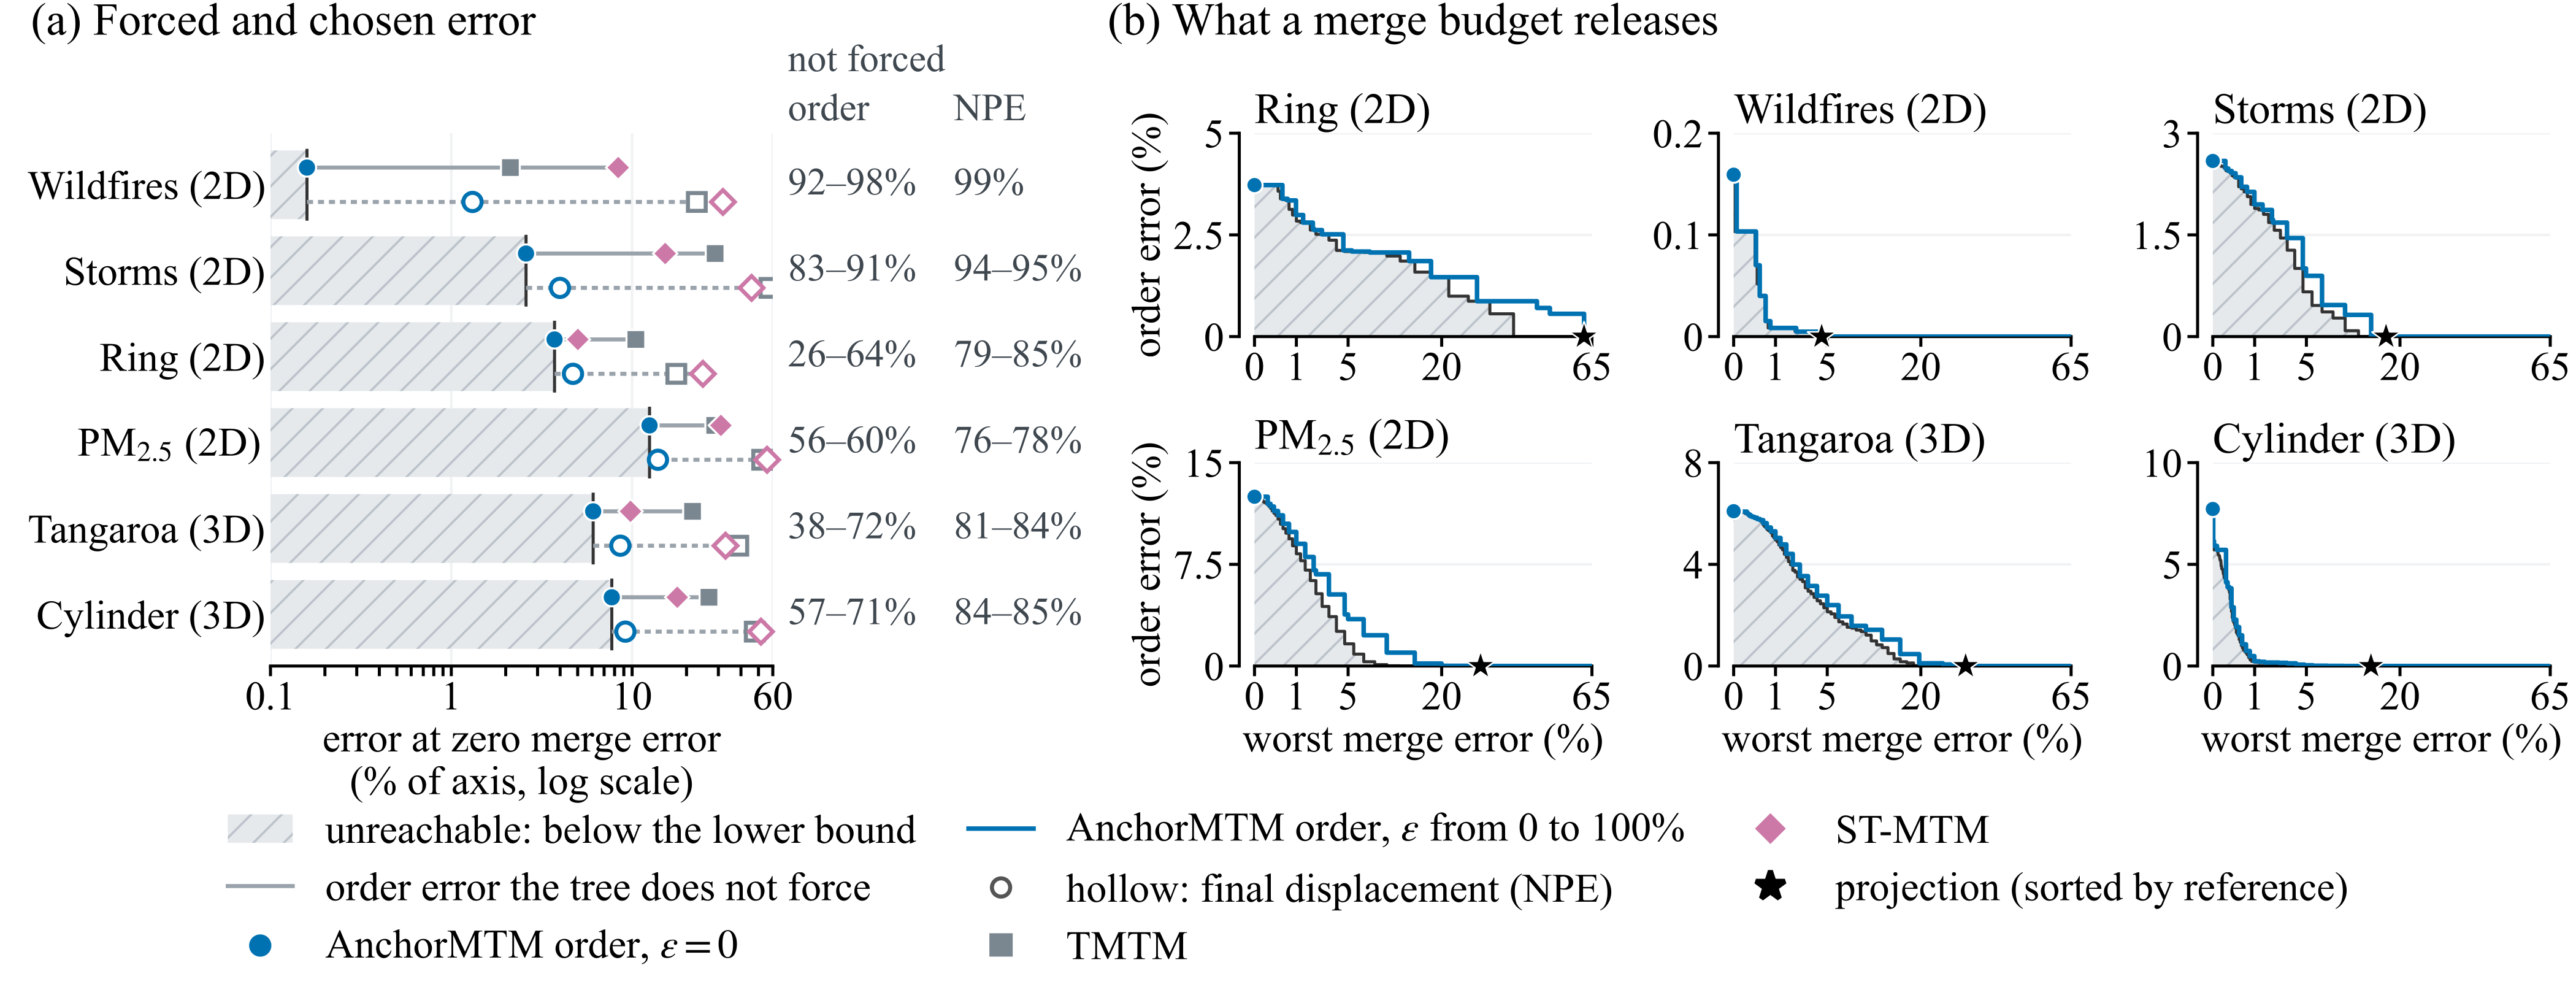
\includegraphics[width=\textwidth]{figures/forced_plane.png}
\caption{Forced and chosen error. (a)~The steps of Section~\ref{sec:bounds} for maps that keep the tree (log scale). The hatched region is what the tree forces: no exact map can lie below the bound $\nu^*$. Filled markers are the order error of each map, hollow markers its final displacement NPE. Midpoint ordering (blue, filled) lies on the bound; TMTM and ST-MTM lie far above it. The right columns give the share of TMTM and ST-MTM error above the point bound, an upper estimate of what a layout with the same widths could remove; Section~\ref{sec:reference-results} gives what Exact removes. (b)~The bound as the merge error grows (Proposition~\ref{thm:chain} and the flattened bound), each panel scaled to its own bound. The budgeted point-model order of AnchorMTM ($\varepsilon$ from 0 to 100\%; worst merge error on a square-root scale) runs along it; the projection keeps every reference but breaks the tree. Bounds and maps use the tolerance $\varepsilon_0$ of Section~\ref{sec:method}.}
\label{fig:plane}
\end{figure*}
\begin{figure*}[!tb]
\paperfigure[\textwidth]{figures/volume_gallery.png}{fig:volume-gallery}{Where each map draws the features of Tangaroa and Cylinder along the streamwise axis; the TMTM, ST-MTM and $\varepsilon=0$ (Exact) columns are the runs of Table~\ref{tab:quantitative-final}. The first column is the reference $q$, the actual location of each feature along $a^*$ and the target of the comparison; light grey dots repeat it in the other panels, and color shows how far a feature is drawn from it. The bars give NPE, the worst displacement of a frame averaged over frames (\% of the axis); for positive budgets, the value in parentheses is the merge error, the largest change of any displayed merge level (\% of the scalar range), a magnitude and not an error rate. TMTM, ST-MTM and Exact show the tree exactly, Exact at the tolerance $\varepsilon_0$ on Cylinder. Each baseline is reflected once to reduce its displacement.}
\end{figure*}
\subsection{Tightness of the Bounds and Forced Error}\label{sec:bounds-eval}
\emph{Controlled trees.} On two sibling pairs below a root, minimax linear programs over all 24 leaf orders, the width-aware bound and the selected order coincide at all 43 overlaps, and all 364 budget tests release the conflict exactly at $2\varepsilon=h$, as Proposition~\ref{thm:chain} predicts.

\emph{Real trees.} The order selected by Exact attains the width-aware bound on 1,271 of 1,560 planar frames, so on these frames no exact-topology order has a smaller worst displacement. Ring attains it on every frame, Wildfires misses one frame and Storms 15. PM$_{2.5}$ attains it on 471 of 744 frames and leaves a small residual gap: the mean interval cost is 13.11\% of the axis against a mean bound of 12.88\%. On the volumes it attains it on 81 of 102 and 68 of 201 frames (Supplementary Section~S4.12).

\emph{Forced and chosen error.} Bounds are evaluated at the tolerance $\varepsilon_0$, as the maps are; on Cylinder, near-equal merge levels lower $\nu^*$ in 34 of 102 frames and its mean from 12.2\% to 7.7\%, and Exact lies above the bound under either reading (Supplementary Section~S4.11). Figure~\ref{fig:plane}a reads the steps of Section~\ref{sec:bounds} for each map. Midpoint ordering attains $\nu^*$ on the same tree, so the step from $\nu^*$ to the order error is chosen by the order rule. On the real-data sequences, 83--98\% of the order error of TMTM and ST-MTM on Wildfires and Storms and 56--60\% on PM$_{2.5}$ lie above $\nu^*$ and could be removed without changing the tree; on the two volumes it is 38--72\%, and on the synthetic Ring 26--64\%. The step from order error to NPE comes from packing and placement: measured in NPE, 76--99\% of the error of TMTM and ST-MTM lies above $\nu^*$. The bounds also reveal how strongly a field entangles its hierarchy with space: $\nu^*$ is 0.16\% of the axis on Wildfires and 2.6\% on Storms, but 12.5\% on PM$_{2.5}$, where nested pollution maxima interleave along the chosen direction. The bound under a merge budget shows what a budget releases (Fig.~\ref{fig:plane}b). Where conflicting subtrees merge just below their parent, little is needed: 1\% removes almost all forced order error on Wildfires (0.16\% to 0.01\%) and on Cylinder (7.7\% to 0.2\%). Where conflicts lie deep, position is expensive: PM$_{2.5}$ needs 10\% to fall below 1\%, and Tangaroa 12\%. The projection reaches zero order error only by changing merge levels by 4--62\% of the scalar range.

\subsection{Position and What It Costs}\label{sec:reference-results}
\emph{Position.} NPE tells whether the anchored axis reaches its goal. Exact lowers NPE relative to TMTM and ST-MTM by 73--96\% on all four planar inputs, from 48--52\% to 9.2\% on Cylinder (at $\varepsilon_0$; 13.6\% strict) and from 33--39\% to 8.6\% on Tangaroa (Table~\ref{tab:quantitative-final}). Balanced, with a budget of at most 10\%, lowers it further on every input. Giving the baselines their best affine map of the axis per sequence, which favors them, still leaves 28--33\% on Tangaroa and 45\% on Cylinder. In Fig.~\ref{fig:volume-gallery}, TMTM and ST-MTM place the features of both volumes in bands that do not follow the references, whereas Exact already reproduces the shedding pattern of Cylinder, and a 5\% budget removes almost all of the rest (NPE 1.2\%). Beyond midpoint ordering, the construction helps mainly under a budget: selective flattening and the search lower $\tau$ by 13--36\% against threshold flattening on PM$_{2.5}$, Wildfires and both volumes, and the final NPE exceeds $\tau$ by at most the slack $\beta_0$ (Supplementary Section~S4.12). Because AnchorMTM optimizes NPE, these results show that the goal is reached, not that AnchorMTM is better in general; the next two paragraphs use measures that do not depend on it.

\emph{Relative geometry.} SNS and TW measure the goal of ST-MTM. At zero budget, ST-MTM has the lower SNS on all four planar inputs and Exact on both volumes; ST-MTM has the higher TW wherever TW is ranked. With a budget, Balanced improves on ST-MTM in SNS and TW on both volumes (TW on Cylinder within 0.001, a 9\% budget on Tangaroa) and in SNS on PM$_{2.5}$, but not on the three benchmark inputs (Table~\ref{tab:quantitative-final}). The higher TW at exact topology follows from what ST-MTM optimizes, not from a weaker pipeline: ST-MTM is another setting of Eq.~\ref{eq:family}. Giving our placement the leaf order of the ST-MTM run, $\lambda_R=0$, no position cap and a stationary temporal target yields TW 0.8925 on Cylinder and 0.8349 on Tangaroa, with NPE back at 48\% and 29\% (Supplementary Section~S4.5). A map that drew every feature exactly at its reference would have TW 0.862 on Cylinder and 0.763 on Tangaroa, below ST-MTM: one spatial axis cannot keep the neighbors of a 2-D or 3-D field, as on all seven sequences of our earlier audit (Supplementary Table~S3). As references, the curves never reach the lowest SNS, but they exceed the TW of every merge tree map on PM$_{2.5}$ and Tangaroa (Hilbert 0.8887 and 0.9222), at the price of the tree.

\emph{Temporal behavior.} On Cylinder, Exact has TD 57 against 43 for ST-MTM. Part of this is real motion, since drawing the references themselves gives 27, and a 10\% budget lowers it to 29; step errors are larger when the displayed order changes (Supplementary Table~S8). On Tangaroa, Exact moves less than ST-MTM (107 against 139). Motion errors (ME) are fewer for Exact than for TMTM and ST-MTM on all seven audit sequences (33\% against 46--67\% on Cylinder, 59\% against 70--97\% on Tangaroa). Exact also reverses fewer displayed steps of matched features (22\% and 19\% of clear steps on Tangaroa and Cylinder, against 39--54\%; Supplementary Section~S4.14).

\begin{figure*}[!tb]
\centering
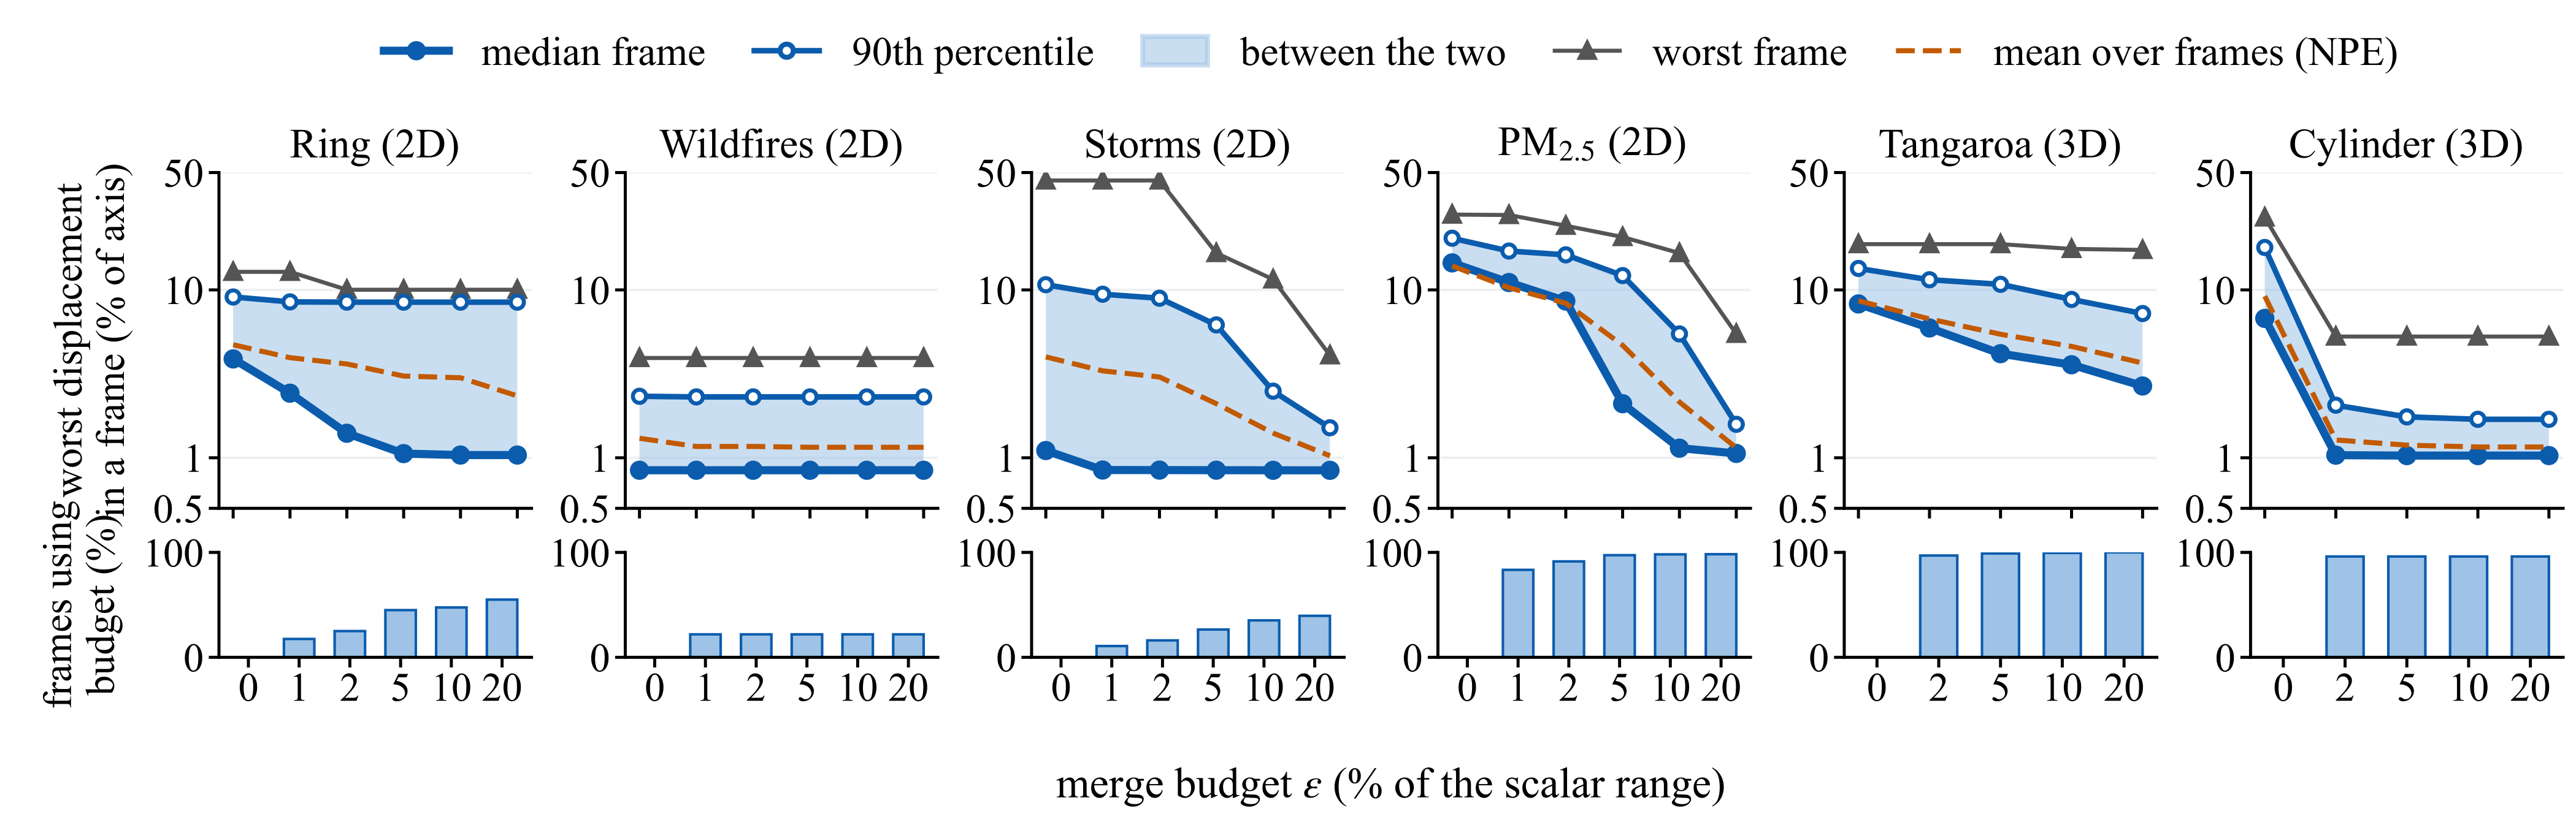
\includegraphics[width=\textwidth]{figures/budget_response_v30.png}
\caption{How a merge budget acts across frames. For each sequence and budget, the worst displacement of every frame is summarized over all frames: the median frame, the 90th percentile and the worst frame (log scale), and the mean over frames, which is NPE (dashed). Bottom: the share of frames whose attained merge error is positive, that is, frames that use the budget. Every frame stays within its budget. The sweep has no 1\% run for the volumes; the 1\% Cylinder run of Table~\ref{tab:quantitative-final} is separate.}
\label{fig:budget-distribution}
\end{figure*}
\subsection{How a Merge Budget Acts across Frames}\label{sec:relaxation-results}
A budget limits merge error, not displacement, so its effect depends on how many frames contain a conflict it can release (Fig.~\ref{fig:budget-distribution}). Two regimes appear. On Storms the budget acts on a tail: 35\% of the frames use the allowance at $\varepsilon=10\%$, the median displacement moves only from 1.10\% to 0.84\%, but the 90th percentile falls from 10.7\% to 2.5\% and the worst frame from 44.8\% to 11.6\%. On PM$_{2.5}$ and the volumes almost every frame contains a releasable conflict and the whole distribution moves: on PM$_{2.5}$, 97\% of the frames use a 5\% budget and the median falls from 14.5\% to 2.1\%; on Cylinder, 2\% already lowers the median from 6.8\% to 1.0\%. Exact has zero merge error on every input, up to $\varepsilon_0$ on Cylinder; Balanced attains at most 0.982, 4.421 and 9.985\% on Ring, Wildfires and Storms.

\begin{figure*}[!tb]
\centering
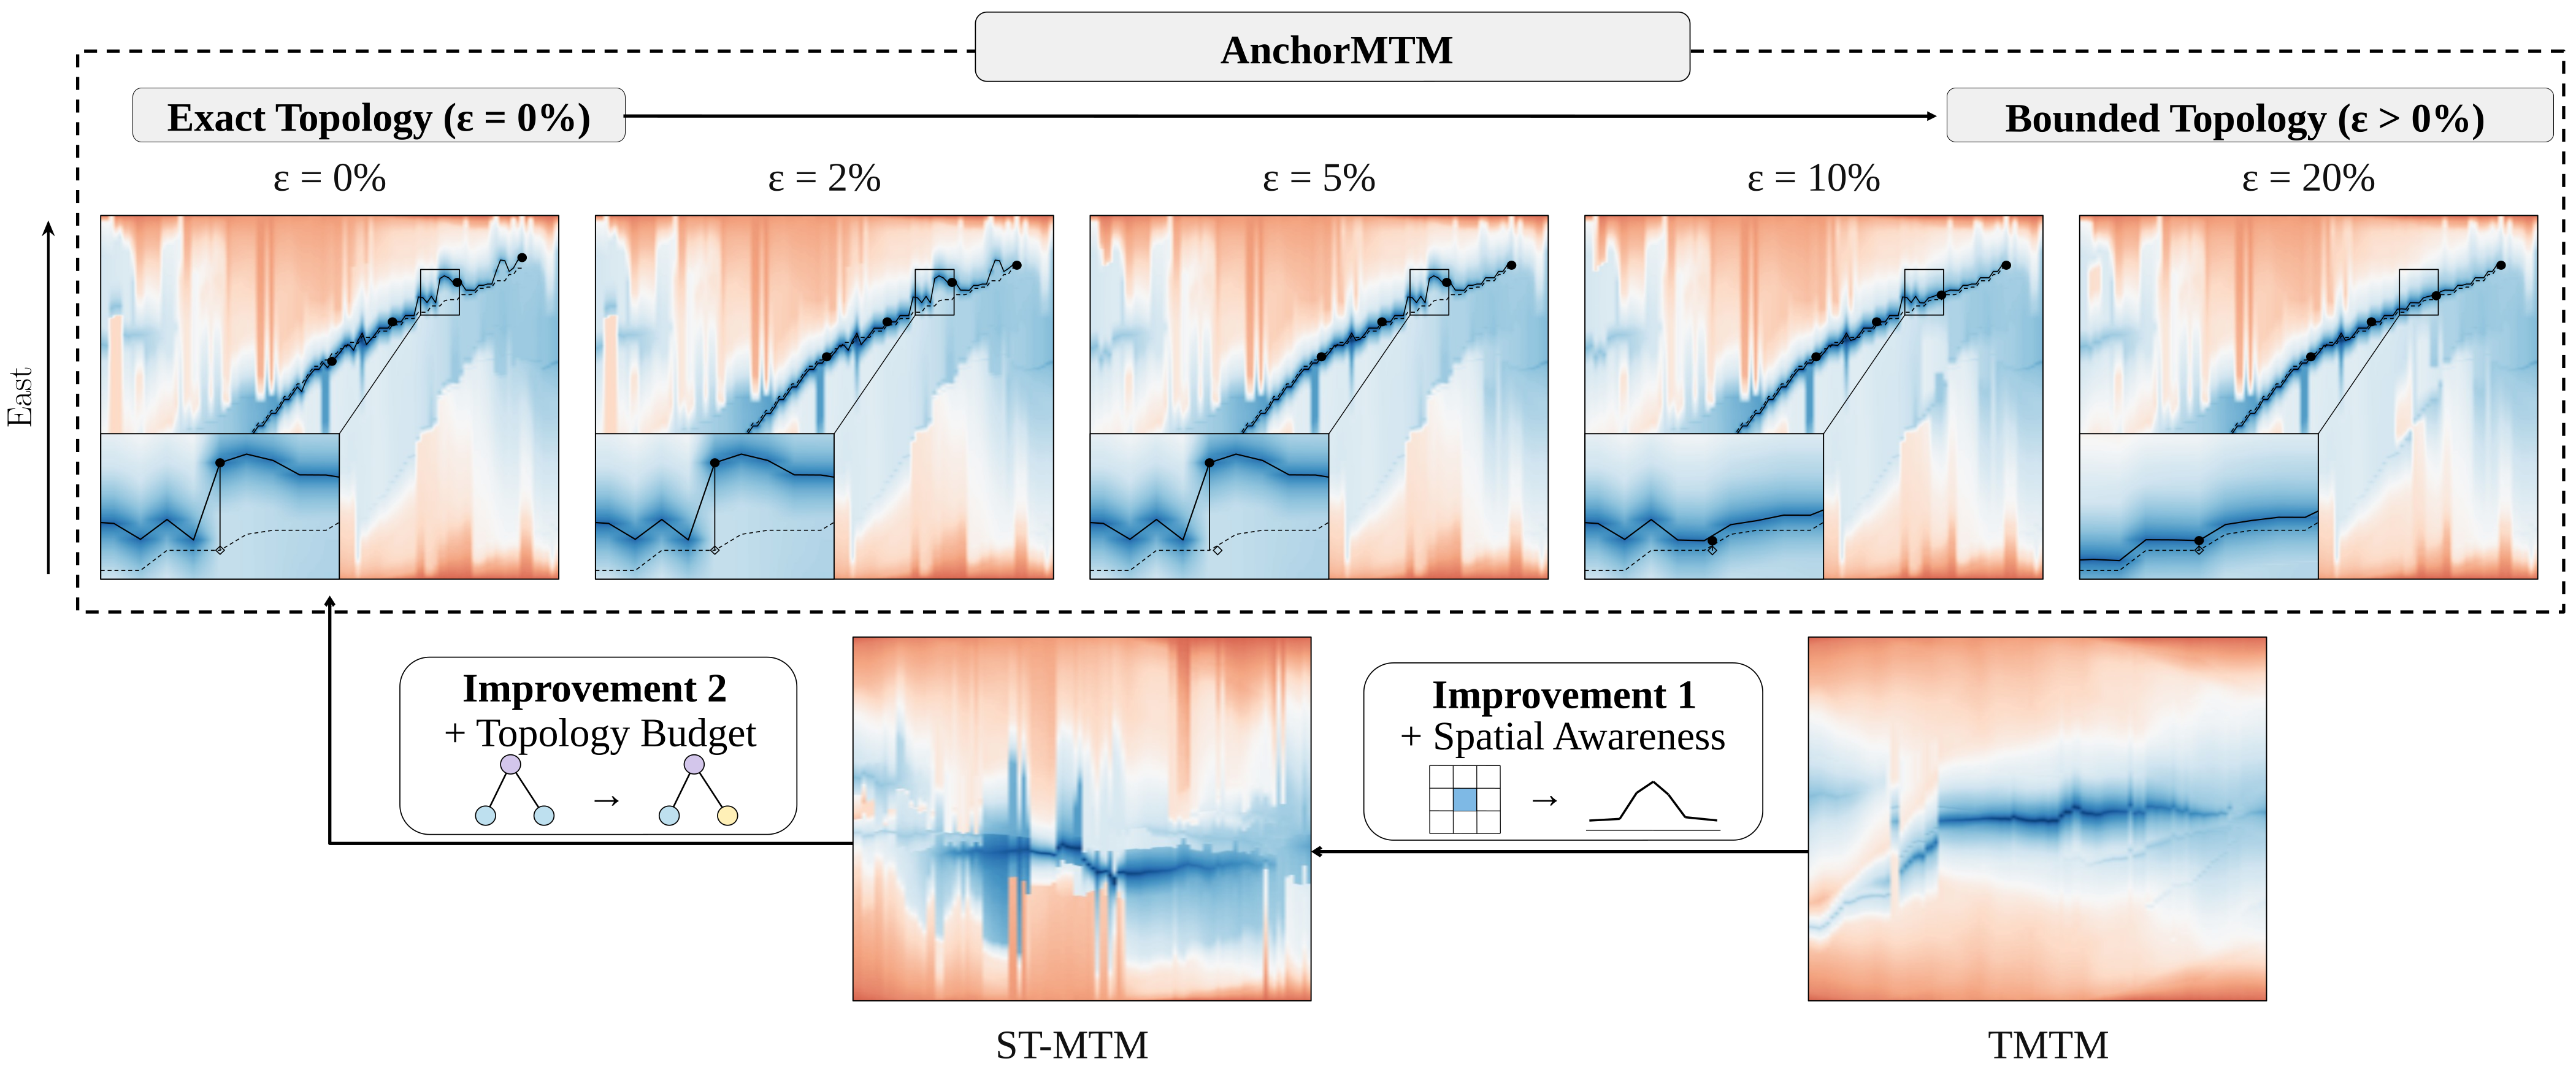
\includegraphics[width=\textwidth]{figures/anchor_storms_budget_maps.png}
\caption{Storms event window, frames 355--460, drawn by AnchorMTM at five budgets and by TMTM and ST-MTM on the same fields and trees, on one $[-35,35]$\,hPa scale. The lower comparison illustrates two improvements: ST-MTM adds pairwise spatial distances to TMTM's tree order, and AnchorMTM gives the axis one fixed direction and controls the merge levels it may change. The dashed curve in the insets is the reference trajectory of the tracked storm; the arrow marks the AnchorMTM axis, from west (bottom) to east (top).}
\label{fig:storms-budget-profiles}
\end{figure*}
\subsection{Case Studies}\label{sec:case-studies}
\paragraph{A storm crossing the North Atlantic.} Between 16 and 19 December 1999, one pressure minimum moves east from the open Atlantic to Scandinavia (snapshots in Fig.~\ref{fig:storms_overview}). AnchorMTM draws this passage as one continuous rising band (Fig.~\ref{fig:storms-budget-profiles}); because the axis runs from west to east, the rise is the eastward motion, and the profile still shows how the low merges with its neighbors. TMTM aligns subtrees by temporal overlap and ST-MTM places them by relative distance, so in both the same low stays at roughly the same height among other changing bands. The axis and the budget act separately: the fixed axis already shows the overall eastward trend at zero budget, and the maps at 0, 2 and 5\% coincide in this window; 10 and 20\% release the remaining conflict, so the segment in the insets follows the reference trajectory more closely.

\paragraph{Vortex shedding behind a cylinder.} The anchored default places the shed vortices at their streamwise positions (Fig.~\ref{fig:volume-gallery}); a hierarchy-guided variant that gives up the spatial axis separates five stages of the wake instead (Supplementary Section~S4.8). Supplementary Fig.~S7 compares the three maps on an hourly PM$_{2.5}$ episode.
